\ifx\allfiles\undefined
\documentclass[12pt, a4paper,oneside, UTF8]{ctexbook}
\usepackage[dvipsnames]{xcolor}
\usepackage{amsmath}   % 数学公式
\usepackage{amsthm}    % 定理环境
\usepackage{amssymb}   % 更多公式符号
\usepackage{graphicx}  % 插图
%\usepackage{mathrsfs}  % 数学字体
%\usepackage{newtxtext,newtxmath}
%\usepackage{arev}
\usepackage{kmath,kerkis}
\usepackage{newtxtext}
\usepackage{bbm}
\usepackage{enumitem}  % 列表
\usepackage{geometry}  % 页面调整
%\usepackage{unicode-math}
\usepackage[colorlinks,linkcolor=black]{hyperref}


\usepackage{ulem}	   % 用于更多的下划线格式,
					   % \uline{}下划线,\uuline{}双下划线,\uwave{}下划波浪线,\sout{}中间删除线,\xout{}斜删除线
					   % \dashuline{}下划虚线,\dotuline{}文字底部加点


\graphicspath{ {flg/},{../flg/}, {config/}, {../config/} }  % 配置图形文件检索目录
\linespread{1.5} % 行高

% 页码设置
\geometry{top=25.4mm,bottom=25.4mm,left=20mm,right=20mm,headheight=2.17cm,headsep=4mm,footskip=12mm}

% 设置列表环境的上下间距
\setenumerate[1]{itemsep=5pt,partopsep=0pt,parsep=\parskip,topsep=5pt}
\setitemize[1]{itemsep=5pt,partopsep=0pt,parsep=\parskip,topsep=5pt}
\setdescription{itemsep=5pt,partopsep=0pt,parsep=\parskip,topsep=5pt}

% 定理环境
% ########## 定理环境 start ####################################
\theoremstyle{definition}
\newtheorem{defn}{\indent 定义}[section]

\newtheorem{lemma}{\indent 引理}[section]    % 引理 定理 推论 准则 共用一个编号计数
\newtheorem{thm}[lemma]{\indent 定理}
\newtheorem{corollary}[lemma]{\indent 推论}
\newtheorem{criterion}[lemma]{\indent 准则}

\newtheorem{proposition}{\indent 命题}[section]
\newtheorem{example}{\indent \color{SeaGreen}{例}}[section] % 绿色文字的 例 ,不需要就去除\color{SeaGreen}{}
\newtheorem*{rmk}{\indent \color{red}{注}}

% 两种方式定义中文的 证明 和 解 的环境:
% 缺点:\qedhere 命令将会失效【技术有限,暂时无法解决】
\renewenvironment{proof}{\par\textbf{证明.}\;}{\qed\par}
\newenvironment{solution}{\par{\textbf{解.}}\;}{\qed\par}

% 缺点:\bf 是过时命令,可以用 textb f等替代,但编译会有关于字体的警告,不过不影响使用【技术有限,暂时无法解决】
%\renewcommand{\proofname}{\indent\bf 证明}
%\newenvironment{solution}{\begin{proof}[\indent\bf 解]}{\end{proof}}
% ######### 定理环境 end  #####################################

% ↓↓↓↓↓↓↓↓↓↓↓↓↓↓↓↓↓ 以下是自定义的命令  ↓↓↓↓↓↓↓↓↓↓↓↓↓↓↓↓

% 用于调整表格的高度  使用 \hline\xrowht{25pt}
\newcommand{\xrowht}[2][0]{\addstackgap[.5\dimexpr#2\relax]{\vphantom{#1}}}

% 表格环境内长内容换行
\newcommand{\tabincell}[2]{\begin{tabular}{@{}#1@{}}#2\end{tabular}}

% 使用\linespread{1.5} 之后 cases 环境的行高也会改变,重新定义一个 ca 环境可以自动控制 cases 环境行高
\newenvironment{ca}[1][1]{\linespread{#1} \selectfont \begin{cases}}{\end{cases}}
% 和上面一样
\newenvironment{vx}[1][1]{\linespread{#1} \selectfont \begin{vmatrix}}{\end{vmatrix}}

\def\d{\textup{d}} % 直立体 d 用于微分符号 dx
\def\R{\mathbb{R}} % 实数域
\def\N{\mathbb{N}} % 自然数域
\def\C{\mathbb{C}} % 复数域
\def\Z{\mathbb{Z}} % 整数环
\def\Q{\mathbb{Q}} % 有理数域
\newcommand{\bs}[1]{\boldsymbol{#1}}    % 加粗,常用于向量
\newcommand{\ora}[1]{\overrightarrow{#1}} % 向量

% 数学 平行 符号
\newcommand{\pll}{\kern 0.56em/\kern -0.8em /\kern 0.56em}

% 用于空行\myspace{1} 表示空一行 填 2 表示空两行  
\newcommand{\myspace}[1]{\par\vspace{#1\baselineskip}}

%s.t. 用\st就能打出s.t.
\DeclareMathOperator{\st}{s.t.}

%罗马数字 \rmnum{}是小写罗马数字, \Rmnum{}是大写罗马数字
\makeatletter
\newcommand{\rmnum}[1]{\romannumeral #1}
\newcommand{\Rmnum}[1]{\expandafter@slowromancap\romannumeral #1@}
\makeatother
\begin{document}
	% \title{{\Huge{\textbf{$Complex \,\, Analysis$\footnote{课堂教材:\textbf{《$Complex \,\, Analysis$》---  $Elias \,\, M. \,\, Stein$}}}}}}
\author{$-TW-$}
\date{\today}
\maketitle                   % 在单独的标题页上生成一个标题

\thispagestyle{empty}        % 前言页面不使用页码
\begin{center}
	\Huge\textbf{序}
\end{center}


\vspace*{3em}
\begin{center}
	\large{\textbf{天道几何,万品流形先自守;}}\\
	
	\large{\textbf{变分无限,孤心测度有同伦。}}
\end{center}

\vspace*{3em}
\begin{flushright}
	\begin{tabular}{c}
		\today \\ \small{\textbf{长夜伴浪破晓梦,梦晓破浪伴夜长}}
	\end{tabular}
\end{flushright}


\newpage                      % 新的一页
\pagestyle{plain}             % 设置页眉和页脚的排版方式(plain:页眉是空的,页脚只包含一个居中的页码)
\setcounter{page}{1}          % 重新定义页码从第一页开始
\pagenumbering{Roman}         % 使用大写的罗马数字作为页码
\tableofcontents              % 生成目录

\newpage                      % 以下是正文
\pagestyle{plain}
\setcounter{page}{1}          % 使用阿拉伯数字作为页码
\pagenumbering{arabic}
\setcounter{chapter}{-1}    % 设置 -1 可作为第零章绪论从第零章开始 
	\else
	\fi
	%  ############################ 正文部分

\chapter{$Week \,\, 9$}
\section{扩充复平面$\hat{\C}$ 上亚纯函数的刻画}
	下面我们将说明,定义在\textbf{扩充复平面$\hat{\C}$} 上的\textbf{亚纯函数}都是\textbf{有理函数}. 在此之前,先来回顾一下\textbf{有理函数}的定义.
	\begin{defn}\label{def 9.1.1}
		A \underline{\textcolor{blue}{\textbf{rational function}}} in $z$ is a quotient of polynomials in $z$.
	\end{defn}

	\vspace{2em}
	这里再来补充一下\textbf{扩充复平面$\C$} 上\textbf{亚纯函数}的定义. (书\footnote{\textbf{《$Complex \,\, Analysis$》---  $Elias \,\, M. \,\, Stein$}}P87,牢林这里又漏了定义!)
	\begin{defn}\label{def 9.1.2}
		A meromorphic function in the complex plane that is either holomorphic at $\infty$ or has a pole at $\infty$ is said to be \underline{\textcolor{blue}{\textbf{meromorphic in the extended complex plane}}}.
	\end{defn}

	\vspace{2em}
	下面给出\textbf{亚纯函数}在\textbf{扩充复平面$\hat{\C}$} 上的刻画.
	\begin{thm}\label{thm 9.1.1}
		The meromorphic functions on $\hat{\C}$ are the rational functions.
		
		\vspace{4em}
		\begin{proof}
			Let $f : \hat{\C} \rightarrow \C$ be a meromorphic function on $\hat{\C}$. Whether $f$ has a pole or removable singularity at $\infty$, $f$ is holomorphic in the set $\{ z \in \C \mid \left| z \right| > R \}$ for some $R$. 
			
			\vspace{1em}
			
			Thus all other possible poles in $\C$ lie in the compact $\{ z \in \C \mid \left| z \right| \leq R \}$, and so $f$ can have only finitely many poles in $\C$, say $z_1 , \cdots , z_k$.\footnote{By \textbf{Bolzano-Weierstrass Theorem}, 任一有界数列必有收敛子列 (高维仍成立), 若poles infinite, 则在紧集$\{ z \in \C \mid \left| z \right| \leq R \}$ 中有聚点, 与meromorphic矛盾.}
			
			\newpage
			
			Hence there are positive numbers $n_1 , \cdots , n_k$, $\st$
			\begin{center}
				$G(z) = (z - z_1)^{n_1} \cdots (z - z_k)^{n_k} f(z)$ has only removable singularities in $\C$.
			\end{center}
		
			\vspace{1em}
			
			After filling the definition of $G$ at $z_1 , \cdots , z_k$, we may assume $G(z)$ is entire. Observe that 
			\begin{center}
				$G(z)$ is rational \hspace*{1em} iff \hspace*{1em} $f(z)$ is rational.
			\end{center}
			For $G(z)$ at $\infty$, there are 3 possibilities:
			
			\vspace{1em}
			
			\begin{enumerate}
				\item[(1)]If $G(z)$ has a pole at $\infty$, then by \textbf{Prop \ref{prop 8.6.1}}, $G(z)$ is a nonconstant polynomial.
				
				\vspace{1em}
				
				\item[(2)]If $G(z)$ has a removable singularity at $\infty$, then $G(z)$ is a constant.
				
				\vspace{1em}
				
				\item[(3)]Assume $\infty$ is an essential singularity of $G(z)$. This is impossible for the Laurent expansion of 
				\begin{align}
					\widetilde{G}(z) \coloneqq G(\frac{1}{z}) = (\frac{1}{z} - z_1)^{n_1} \cdots (\frac{1}{z} - z_k)^{n_k} f(\frac{1}{z}) \,\, \text{near the origin}
				\end{align}
				has only finitely negative powers. Thus $\infty$ is not an essential singularity of $G(z)$.
			\end{enumerate}
		
			\vspace{1em}
			
			Therefore, $G(z)$ is rational, then $f(z)$ is rational.
		\end{proof}
	\end{thm}

\newpage
\section{辐角原理,Rouch\'{e}'s Theorem}
\subsection{$The \,\, Argument \,\, Principle$}
	下面给出\textbf{辐角原理}的叙述.
	\begin{thm}\label{thm 9.2.1}
		\textbf{Argument Principle}. \\
		Suppose $f$ is meromorphic in an open set containing a contour $\gamma$ and its interior. If $f$ has no poles and never vanishes on $\gamma$, then
		\begin{align}
			\frac{1}{2 \pi i} \int_{\gamma}{\frac{f^{'}(z)}{f(z)} dz}
			= \# \left( \text{zeros of $f$ in Interior($\gamma$)} \right) - \# \left( \text{poles of $f$ in Interior($\gamma$)} \right)
		\end{align}
		where the zeros and poles are counted with their multiplicaties (i.e. orders).
		
		\vspace{2em}
		
		\begin{rmk}
			可从\textbf{几何视角}来看待\textbf{辐角原理}. \\
			函数$f$ 实际上引导了一个复平面$z-plane$ 到另一个复平面$w-plane$ 的变换,即
			\begin{center}
				The mapping $w = f(z)$ maps the contour $\gamma$ to a closed path $\Gamma$ in $w-plane$.
			\end{center}
			
			\begin{figure}[htbp]  %h此处,t页顶,b页底,p独立一页,浮动体出现的位置
				\centering  %图表居中
				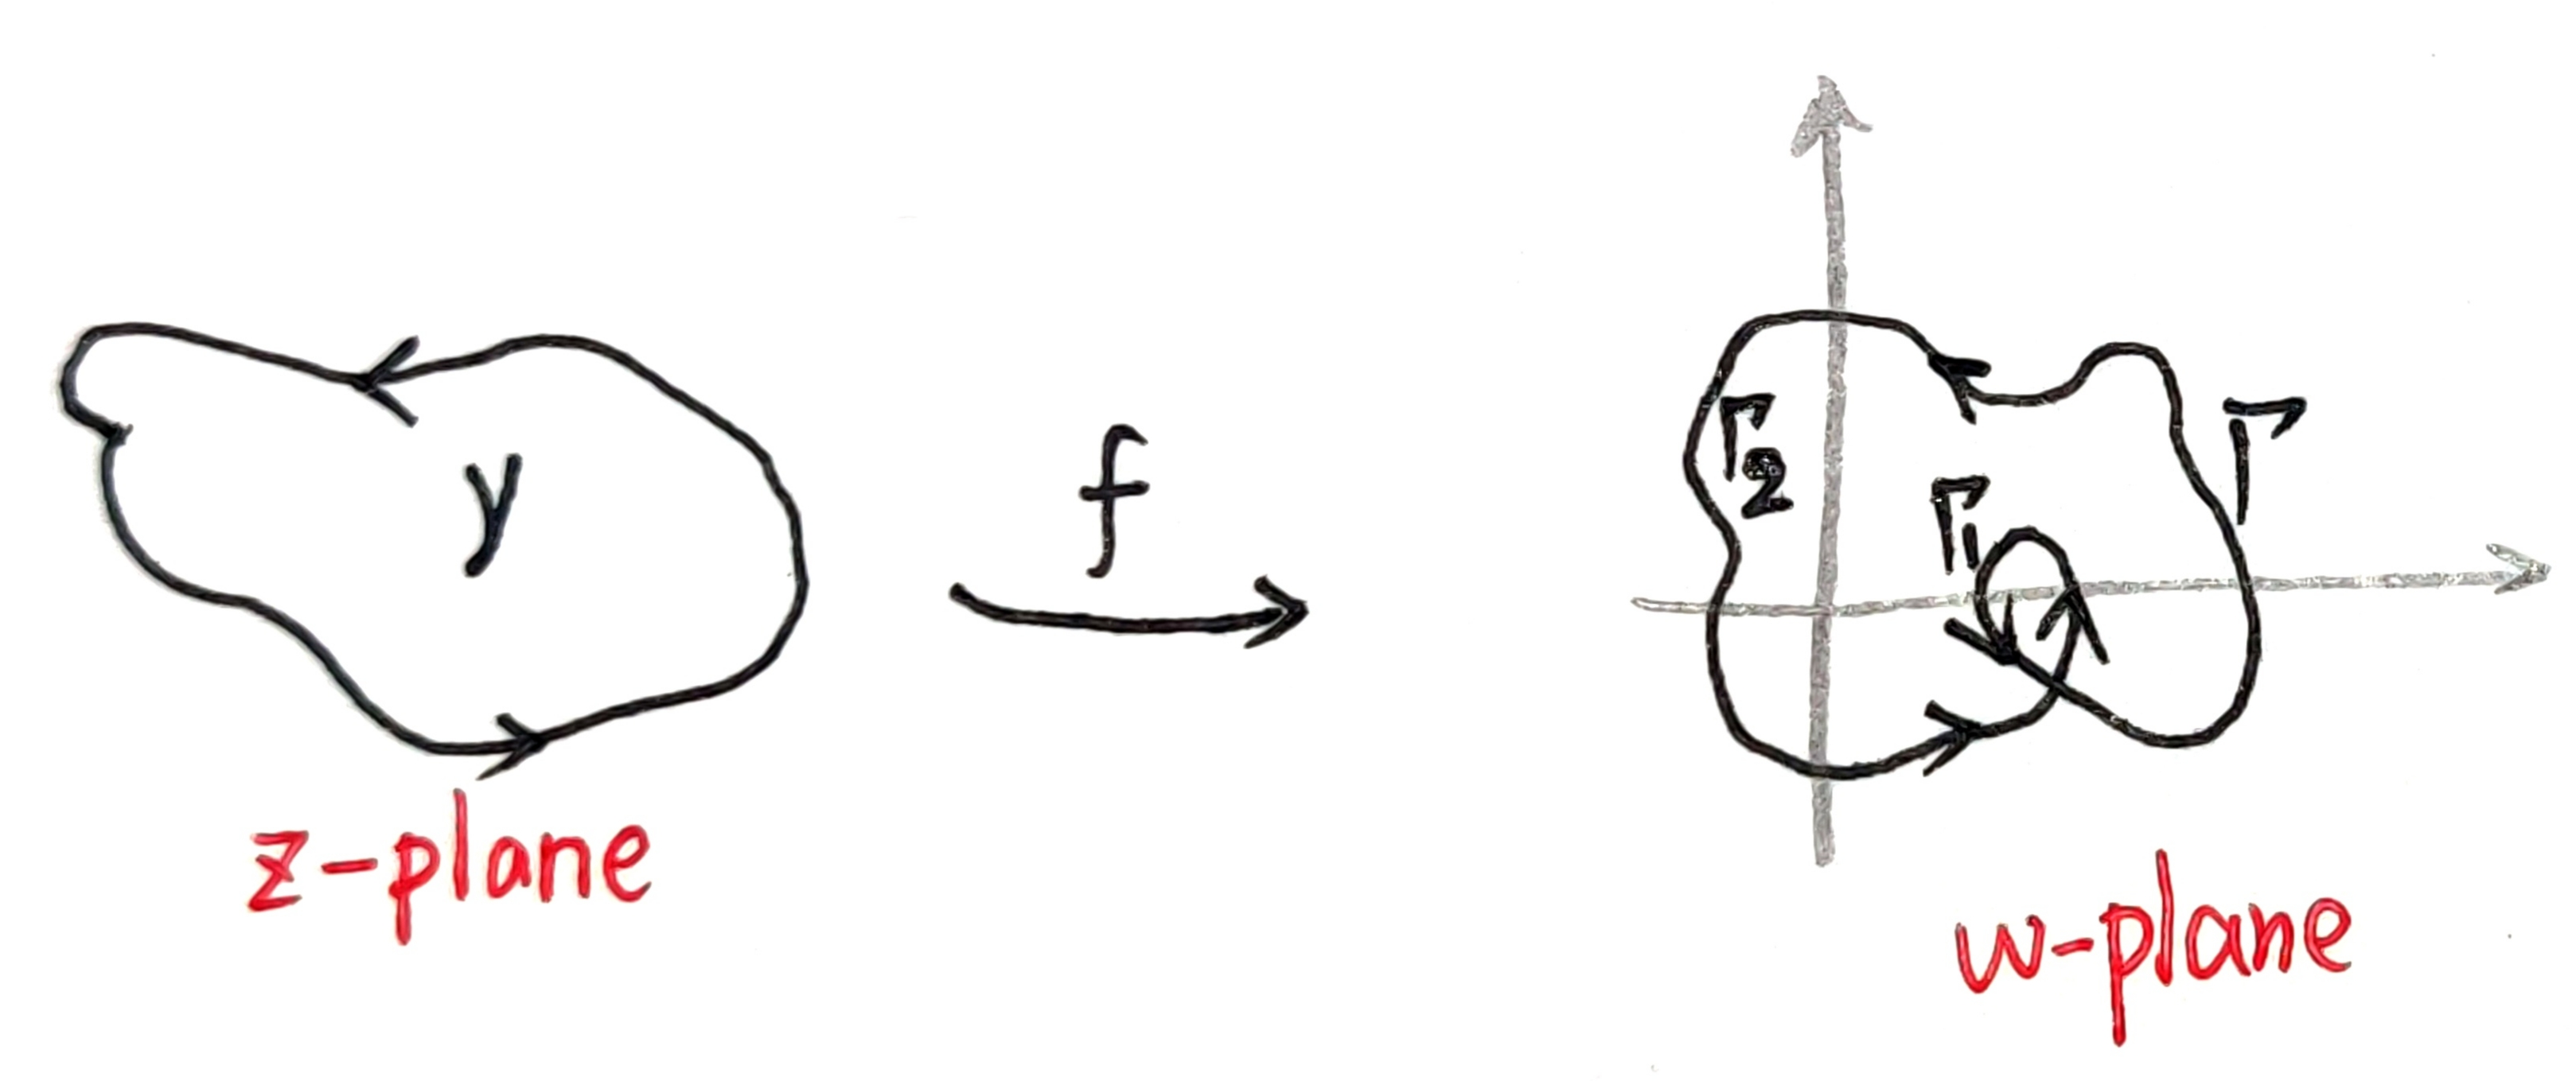
\includegraphics[width=0.5\textwidth]{figure/9.2.1-1} %图片的名称或者路径之中有空格会出问题 
				\caption{mapping $w = f(z)$} % 图片标题
				\label{pic 9.2.1-1}
			\end{figure}
			
			Let $\Gamma(t) = (f \circ \gamma)(t) = f(\gamma(t))$, $t \in [0 , 1]$. Then
			\begin{align}
				\frac{1}{2 \pi i} \int_{\gamma}{\frac{f^{'}}{f} dz}
				= \frac{1}{2 \pi i} \int_{\Gamma}{\frac{dw}{w}}
			\end{align}
			闭曲线$\Gamma$可拆为若干简单闭曲线,即
			\begin{center}
				$\Gamma = \Gamma_1 + \cdots + \Gamma_k$
			\end{center}
			\begin{itemize}
				\item 若$\Gamma_i$ 内部无原点,则$\frac{1}{w}$ holomorphic,$\int_{\Gamma_i}{\frac{dw}{w}} = 0$.
				
				\item 若$\Gamma_i$ 内部有原点,则$\int_{\Gamma_i}{\frac{dw}{w}} = 2 \pi i$.
			\end{itemize}
			从而
			\begin{align}
				\frac{1}{2 \pi i} \int_{\gamma}{\frac{f^{'}}{f} dz}
				= \frac{1}{2 \pi i} \int_{\Gamma}{\frac{dw}{w}}
				= \text{$\Gamma$ 绕原点圈数}
			\end{align}
		\end{rmk}
	
		\newpage
		
		\begin{proof}
			Let $f \not\equiv 0$ (不恒为0) be a meromorphic function on an open set $\Omega$. 
			
			\vspace{2em}
			
			\begin{itemize}
				\item If $f$ has a pole of order $n$ at $\alpha \in \Omega$, then by \textbf{Thm \ref{thm 7.1.2}}, $\exists$ a nonvanishing (恒不为0) holomorphic function $h(z)$ in a neighbourhood of $\alpha$, $\st$
				\begin{center}
					$f(z) = (z - \alpha)^{-n} h(z)$
				\end{center}
				Then
				\begin{align}
					\frac{f^{'}(z)}{f(z)} &= -\frac{n}{z - \alpha} + \frac{h^{'}(z)}{h(z)} \\
					Res_{\alpha}\frac{f^{'}}{f} &= -n = - \,\, \text{the order of the pole $\alpha$ of $f$}
				\end{align}
				
				\vspace{2em}
				
				\item If $\beta \in \Omega$ is a zero of order $m$ of $f$, then by \textbf{Thm \ref{thm 7.1.1}}, $\exists$ a nonvanishing holomorphic function $g(z)$ in a neighbourhood of $\beta$, $\st$
				\begin{center}
					$f(z) = (z - \beta)^{m} g(z)$
				\end{center}
				Then
				\begin{align}
					\frac{f^{'}(z)}{f(z)} &= \frac{m}{z - \beta} + \frac{g^{'}(z)}{g(z)} \\
					Res_{\beta}\frac{f^{'}}{f} &= m = \text{the order of the zero $\beta$ of $f$}
				\end{align}
			\end{itemize}
			
			\vspace{2em}
			
			Therefore, $\frac{f^{'}}{f}$ has simple poles at the zeros and poles of $f$, and
			\begin{align}
				\frac{1}{2 \pi i} \int_{\gamma}{\frac{f^{'}(z)}{f(z)} dz}
				= \# \left( \text{zeros of $f$ in Interior($\gamma$)} \right) - \# \left( \text{poles of $f$ in Interior($\gamma$)} \right)
			\end{align}
			where the zeros and poles are counted with their multiplicaties (i.e. orders).
		\end{proof}
	\end{thm}

\newpage
\subsection{Rouch\'{e}'s Theorem}
	作为\textbf{辐角原理}的推论,下面给出这个强有力的工具\textbf{Rouch\'{e}'s Theorem}.
	\begin{thm}\label{thm 9.2.2}
		\textbf{Rouch\'{e}'s Theorem}. \\
		Suppose $f , g$ are holomorphic in an open set containing a contour $\gamma$ and its interior. If $\left| f(z) \right| > \left| g(z) \right|$ for all $z \in \gamma$, then
		\begin{center}
			$f$ and $f \pm g$ have the same number of zeros in Interior($\gamma$).
		\end{center}
	
		\vspace{2em}
		\begin{proof}
			详细证明可见书\footnote{\textbf{《$Complex \,\, Analysis$》---  $Elias \,\, M. \,\, Stein$}}P91 Thm 4.3.
		\end{proof}
	\end{thm}

	\vspace{2em}
	利用\textbf{Rouch\'{e}'s Theorem},我们可以证明许多结论,比如\textbf{代数基本定理 (FTA, $\S$9.3 题2)}.
	
	

\newpage
\section{课堂例题$2024-04-22$}
	\begin{enumerate}
		\item Determine the number of zeros of
		\begin{center}
			$p(z) = z^7 + 5z^3 - z - 2$ in $\mathbb{D}$
		\end{center}
	
		\vspace{2em}
		\begin{solution}
			Let $f(z) = 5z^3$, $g(z) = z^7 - z - 2$. Then $\left| f(z) \right| = 5 > 4 \geq \left| g(z) \right|$ on $z \in \partial \mathbb{D}$. \\
			Therefore, by \textbf{Rouch\'{e}'s Theorem (Thm \ref{thm 9.2.2})},
			\begin{center}
				$p(z) = f(z) + g(z)$ has the same number of zeros as $f$ in $\mathbb{D}$, which is 3.
			\end{center}
		\end{solution}
	
		\vspace{6em}
		
		\item \textbf{(代数基本定理, FTA)} \\
		Let $p(z) = z^n + a_1 z^{n - 1} + \cdots + a_{n - 1}z + a_n$, where $a_1 , \cdots , a_n \in \C$. Then
		\begin{center}
			$p(z)$ has $n$ zeros in $\C$.
		\end{center}
	
		\vspace{2em}
		\begin{solution}
			Let $f(z) = z^n$, $g(z) = a_1 z^{n - 1} + \cdots + a_{n - 1} z + a_n$. \\
			If $R$ is sufficiently large, say $R > \max{\left\{ 1 , n \cdot \max_{1 \leq k \leq n}{\left| a_k \right|} \right\}}$, then
			\begin{center}
				$\left| f(z) \right| > \left| g(z) \right|$ for all $z \in C_{R}(0)$
			\end{center}
			Therefore, by \textbf{Rouch\'{e}'s Theorem (Thm \ref{thm 9.2.2})},
			\begin{center}
				$p(z) = f(z) + g(z)$ has the same number of zeros as $f$ in $\C$, which is $n$.
			\end{center}
		\end{solution}
	
		\newpage
		
		\item \textbf{(书P26 题7)} \\
		Suppose $\left| a_k \right| < 1$, $k = 1 , 2 , \cdots , n$.
		\begin{align}
			f(z) = \prod_{k = 1}^{n}{\frac{z - a_k}{1 - \overline{a_k}z}}
		\end{align}
		If $\left| b \right| < 1$, then $f(z) = b$ has $n$ roots in $\mathbb{D}$.
		
		\vspace{2em}
		\begin{proof}
			Let $g(z) = b$. Then $\left| g(z) \right| = \left| b \right| < \left| f(z) \right| = 1$ for all $z \in \partial \mathbb{D}$. \\
			Then by \textbf{Rouch\'{e}'s Theorem (Thm \ref{thm 9.2.2})},
			\begin{center}
				$f(z) - b = f(z) - g(z)$ has the same number of zeros as $g$ in $\mathbb{D}$, which is 0.
			\end{center}
		\end{proof}
	\end{enumerate}
	






	%  ############################
	\ifx\allfiles\undefined
\end{document}
\fi